%------------------------------------------------
\section{Introducción} 
%------------------------------------------------

\subsection{Motivación}

\begin{frame}
	\frametitle{Introducción}
		\begin{columns}[T]
            \begin{column}{.60\textwidth}
                      \begin{block}{Motivación}
                        \begin{itemize}
                                 \item Larga espera.
                                 \item Optimización del control de paso.
                                 \item Peatones.
                                 \item Reducción de consumo.
                                 \item Contaminación ambiental.
                         \end{itemize}
                \end{block}
              \end{column}
              \hfill
            \begin{column}{.40\textwidth}

                     \begin{figure}[htbp]
                                \centering
                                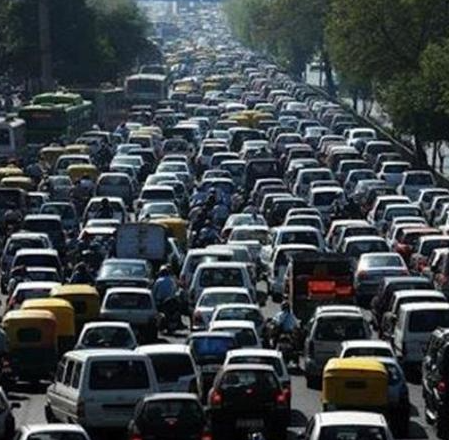
\includegraphics[width=1\textwidth]{diagramas/motivacion.png}
                        \end{figure}

               \end{column}
      \end{columns}
	\end{frame}

\subsection{Antecedentes}

\begin{frame}
\frametitle{Introducción}
\begin{block}{Antecedentes}
	\begin{itemize}
		\item Róterdam, Holanda: Calles equipadas con sensores de temperatura que detectan el grado de calor derivado del número de bicis que se acercan.
		\item Brasil: Google Maps para ver dónde hay más vehículos y dejar la señal de verde por más tiempo en esos tramos.
		\item Holanda: Intersecciones equipadas con LEDs en el pavimento para los peatones que cruzan distraídos con el celular.
	\end{itemize}

       \begin{figure}[htbp]
               \centering
               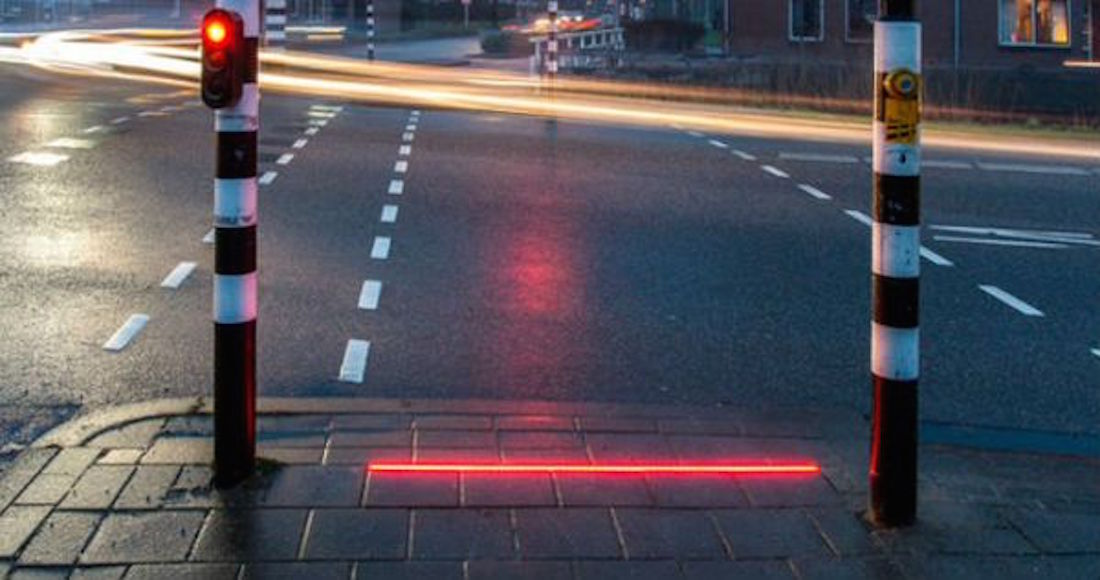
\includegraphics[width=0.5\textwidth]{diagramas/antecedente1.jpg}
       \end{figure}
\end{block}
\end{frame}

%------------------------------------------------
\section{Modelado y abstracción}
%------------------------------------------------

\begin{frame}
\frametitle{Modelado y abstracción}
\begin{block}{}
	\begin{itemize}
		\item Modelo de intersección entre dos avenidas.
		\item Sensores de proximidad que simulan la presencia de autos en cada tramo.
		\item Tareas que controlan el comportamiento de cada semáforo.
		\item La intersección es el recurso compartido entre todas las tareas.
		\item Los accesos deben serializarse.
		\item Primitivas de sincronización (mutexes).
		\item El sistema debe responder a diferentes casos generales.
	\end{itemize}
\end{block}
\end{frame}

\begin{frame}
\frametitle{Todos los tramos inactivos}
	\begin{figure}[htbp]
		\centering
		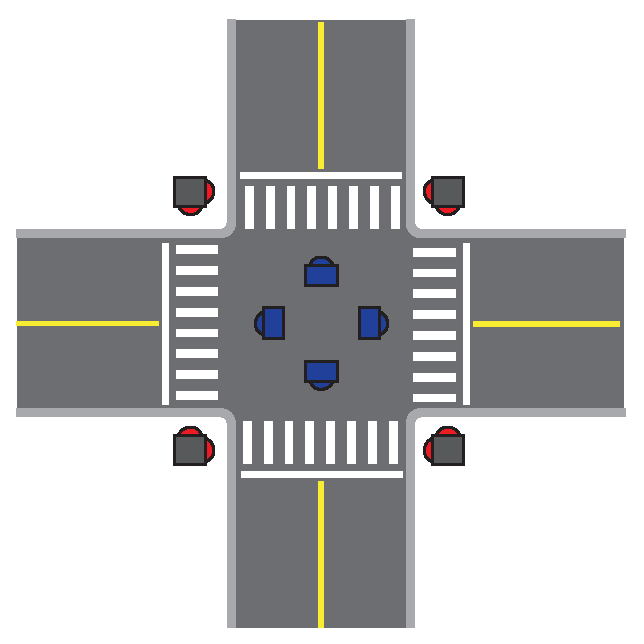
\includegraphics[width=0.750\textwidth]{diagramas/ningun-activo.eps}
	\end{figure}
	%El sistema debe responder haciendo Round-Robin entre todos los semáforos inactivos.
\end{frame}

\begin{frame}
\frametitle{Un tramo activo}
\begin{figure}[htbp]
	\centering
	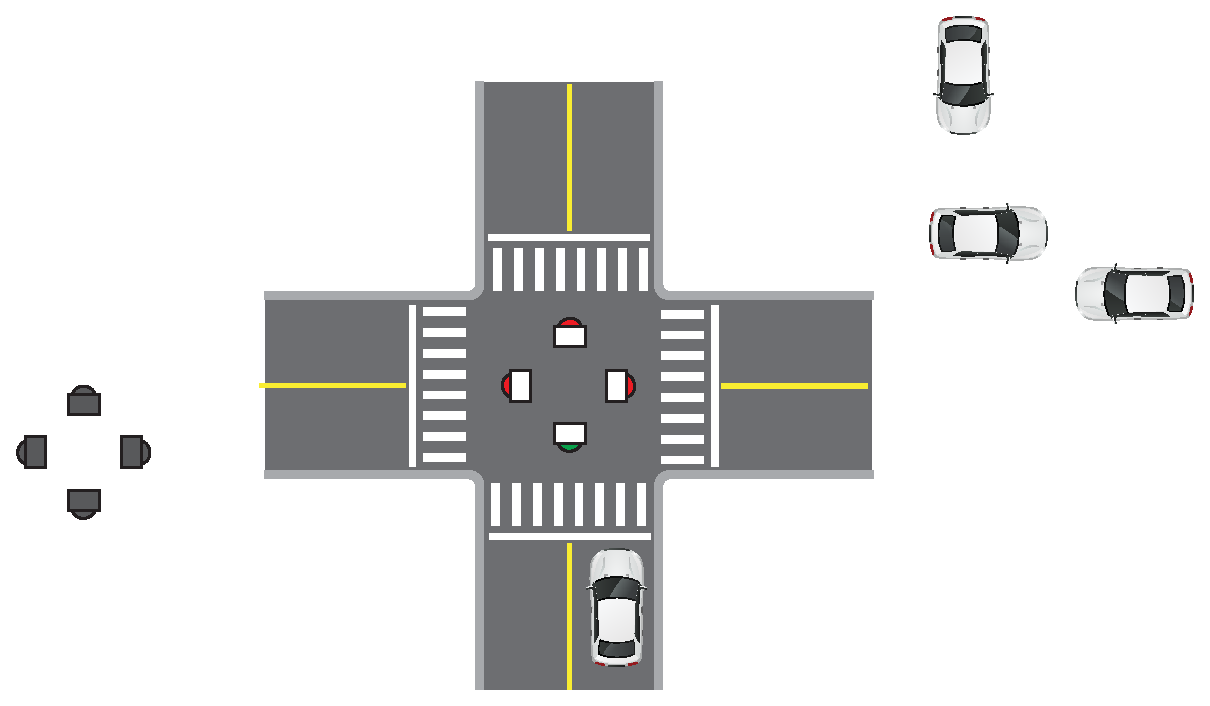
\includegraphics[width=0.750\textwidth]{diagramas/un-activo.eps}
\end{figure}
%El sistema debe otorgarle verde sólo al semáforo activo.
\end{frame}

\begin{frame}
\frametitle{Más de un tramo activo}
\begin{figure}[htbp]
	\centering
	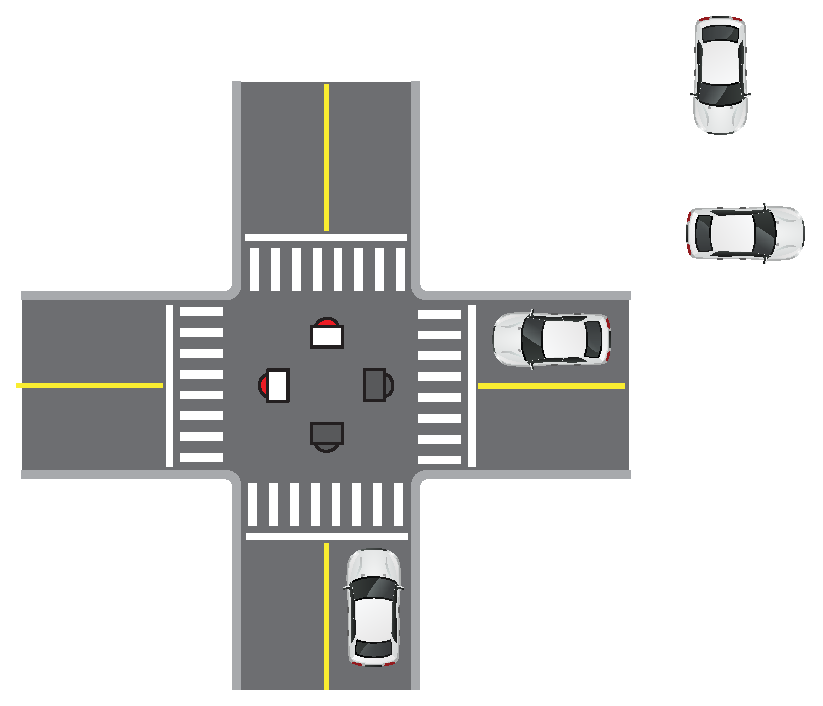
\includegraphics[width=0.750\textwidth]{diagramas/dos-activos.eps}
\end{figure}
%El sistema debe responder haciendo Round-Robin sólo entre los semáforos activos.
\end{frame}

\begin{frame}
\frametitle{Todos los tramos activos}
\begin{figure}[htbp]
	\centering
	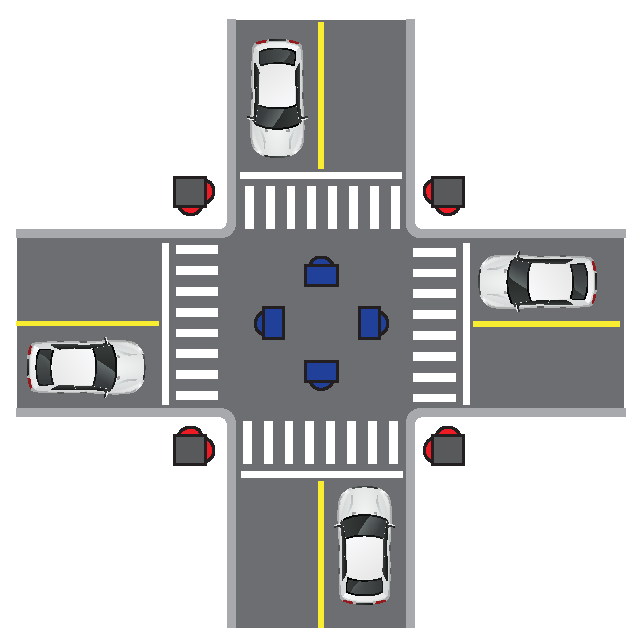
\includegraphics[width=0.750\textwidth]{diagramas/todos-activos.eps}
\end{figure}
%El sistema debe responder haciendo Round-Robin entre todos los semáforos.
\end{frame}

\begin{frame}
\frametitle{Interacción con peatones}
\begin{figure}[htbp]
	\centering
	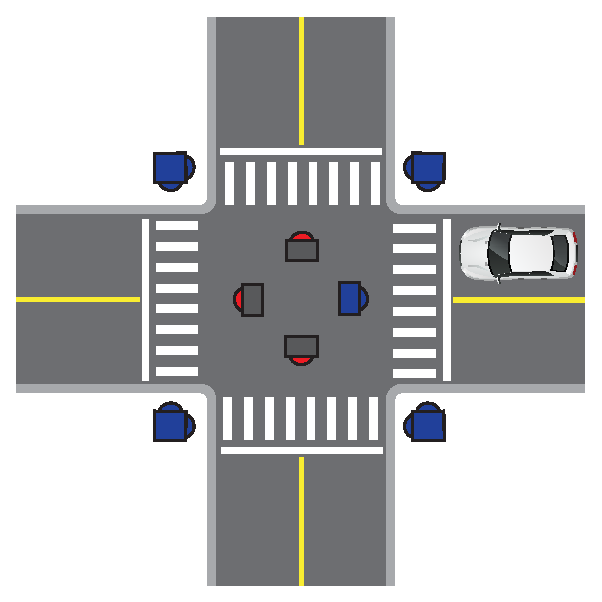
\includegraphics[width=0.750\textwidth]{diagramas/peaton-auto.eps}
\end{figure}
%La pulsación del botón le indica al sistema que por una única vez se le debe dar paso al peatón y luego se continúa de acuerdo a la actividad de cada tramo.
\end{frame}

%------------------------------------------------
\section{Implementaciones}
%------------------------------------------------

\begin{frame}
\frametitle{Plataforma de desarrollo}
\begin{block}{}
	\begin{itemize}
		\item Implementación sobre la plataforma Arduino.
		\item Implementación no oficialmente soportada de FreeRTOS. \href{https://github.com/feilipu/Arduino/FreeRTOS/Library}{https://github.com/feilipu/Arduino/FreeRTOS/Library}
	\end{itemize}

\begin{columns}[T]
	\begin{column}{.50\textwidth}
	\begin{figure}[htbp]
		\centering
		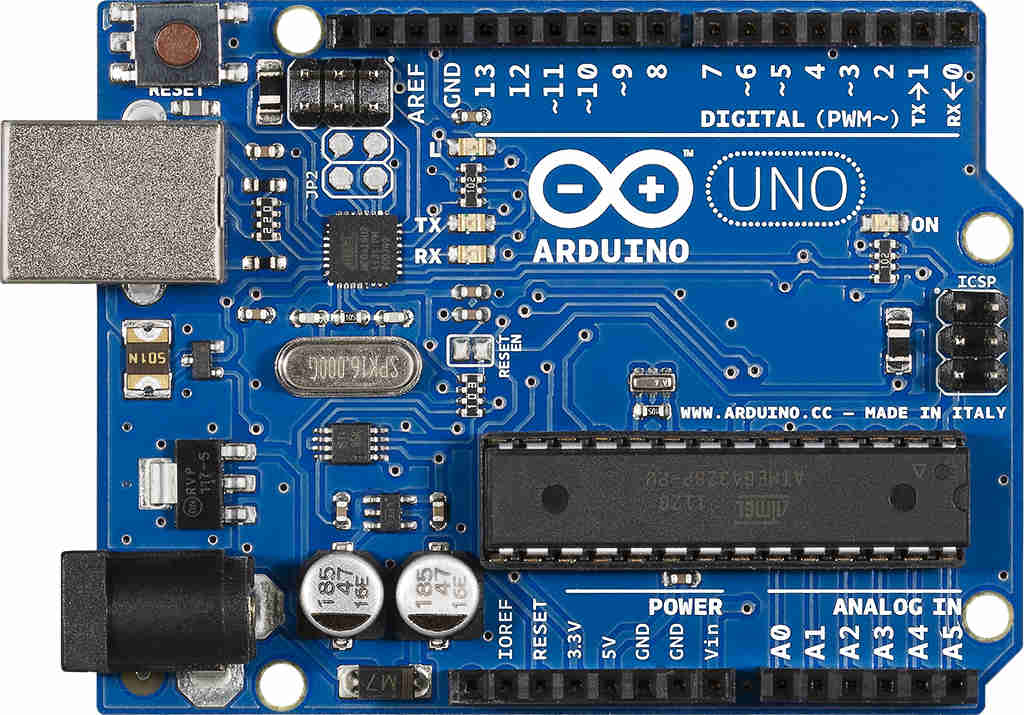
\includegraphics[width=1\textwidth]{diagramas/implementacion1.jpg}
	\end{figure}
	\end{column}
	\hfill
	\begin{column}{.50\textwidth}
		
		\begin{figure}[htbp]
			\centering
			
\includegraphics[width=1\textwidth]{diagramas/implementacion2.jpg}
		\end{figure}
		
	\end{column}
\end{columns}
\end{block}
\end{frame}

\subsection{Primera implementación}

\begin{frame}
\frametitle{Implementación A}
\begin{block}{Única sección crítica con una clase controlador}
	\begin{itemize}
		\item Planificación a cargo de una tarea de alta prioridad.
		\item Una tarea a cargo del sensado del tráfico, también de alta prioridad.
		\item Diferentes prioridades estáticas.
		\item Gran cantidad de tareas corriendo en simultáneo.
		\item Modelo productor-consumidor para el pasaje de datos.
	\end{itemize}
\end{block}
\begin{block}{Problemas de esta implementación}
	\begin{itemize}
		\item Poca escalabilidad.
		\item Dificultad para considerar un semáforo para peatones.
		\item En rojo todos los semáforos, cuando todos los tramos están inactivos.
		%\item Debido a las prioridades estáticas, cuando todos los tramos están inactivos, no se puede realizar el Round-Robin%
	\end{itemize}
\end{block}
\end{frame}

\subsection{Implementación B}
\begin{frame}
\frametitle{Implementación B}
\begin{block}{Única sección crítica sin una clase controlador}
	\begin{itemize}
		\item Planificación a cargo del scheduler de FreeRTOS.
		\item Prioridades variables a lo largo del tiempo.
		\item Admite fácilmente un semáforo que controle la circulación de los peatones.
		\item Una tarea por semáforo más una tarea de sensado para el botón para peatones.
		\item Fácil de añadir más semáforos.
		\item Grave problema con el cambio de prioridades sobre tareas bloqueadas.
	\end{itemize}
\end{block}
\end{frame}

\subsection{Problemas de la implementación B}
\begin{frame}
\frametitle{Problemas de la implementación B}
\begin{block}{}
	\begin{itemize}
		\item El planificador no se comporta como se esperaba.
		\item El orden del Round-Robin está dado por el orden en que se bloquean las tareas. Existe un workaround.
		\item El cambio de prioridad de tareas bloqueadas se retrasa.
		\item Posible bug en el port de FreeRTOS para Arduino (Se tomó como referencia una implementación simulada de FreeRTOS para Win32).
	\end{itemize}
\end{block}
\end{frame}

\subsection{Implementación C}
\begin{frame}
\frametitle{Implementación C}
\begin{block}{Múltiples secciones críticas y sistema basado en turnos.}
	\begin{itemize}
		\item Cada semáforo se duerme en su propio mútex.
		\item Prioridades fijas.
		\item Pocas tareas ejecutándose concurrentemente.
		\item Fácil de expandir.
		\item Permite fácilmente agregar el control del peatón como si fuese otro semáforo más.
		\item Utilización de la técnica \emph{passing the baton}.
	\end{itemize}
\end{block}
\end{frame}

%------------------------------------------------
\section{Conclusiones}
%------------------------------------------------

\subsection{Conclusiones}
\begin{frame}
	\begin{block}{Conclusiones}
		\begin{itemize}
			\item Los cambios de prioridades de tareas en estado bloqueadas no son inmediatos.
			\item El orden del Round-Robin del scheduler no es configurable.
			\item La implementación no oficial de FreeRTOS para Arduino puede tener problemas al manejar prioridades.
		\end{itemize}
	\end{block}
\end{frame}